\subsection{Програмна реалізація модуля автоматизованого тестування}

Основним інструментом для проведення тестування якості масштабування є функція \texttt{runBenchmark}. Програмний код модуля поєднує в собі логіку обходу файлової системи та динамічного оновлення графічного інтерфейсу користувача.

\paragraph{Режими запуску тестування.}
Для забезпечення гнучкості під час проведення експериментів, графічний інтерфейс програми підтримує три різні сценарії запуску тестування:
\begin{itemize}
	\item \textbf{На поточному зображенні:} розрахунок метрик виконується виключно для того файлу, який наразі відкрито у робочому просторі програми.
	\item \textbf{Вибір зображення:} користувач має змогу через стандартний файловий діалог вказати конкретне зображення на диску для проведення ізольованого тесту.
	\item \textbf{Вибір директорії:} режим обробки який дозволяє обрати цілу папку. Програма автоматично зчитає всі файли у вказаній директорії, що є критично важливим для збору об'єктивної статистики на великих датасетах.
\end{itemize}
Вибір відповідного режиму здійснюється через спеціальний розділ головного меню програми (рис.~\ref{fig:testing_modes_menu}).

\newpage
\begin{figure}[htbp]
	\centering
	% Вкажи правильний шлях до скриншота меню з вибором режимів
	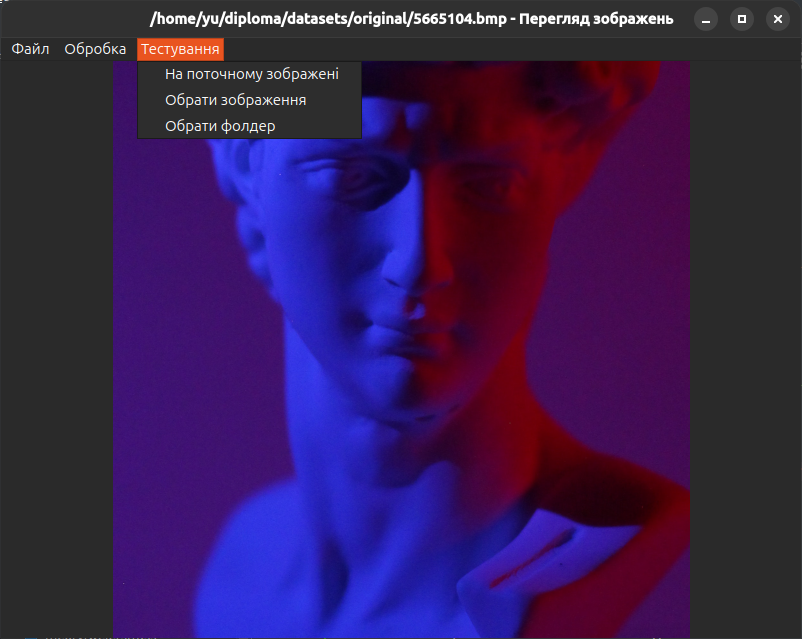
\includegraphics[width=0.8\textwidth]{figures/test}
	\caption{Меню вибору режиму автоматизованого тестування}
	\label{fig:testing_modes_menu}
\end{figure}

\paragraph{Конфігурація параметрів тестування.}
Одразу після вибору джерела вхідних даних (поточне зображення, окремий файл або ціла директорія) програма ініціює спеціальне діалогове вікно. У цьому вікні користувачу надається можливість налаштувати умови поточного експерименту (рис.~\ref{fig:test_config_dialog}).

\begin{figure}[htbp]
	\centering
	% Вкажи правильний шлях до скриншота конфігураційного вікна (твоє останнє фото)
	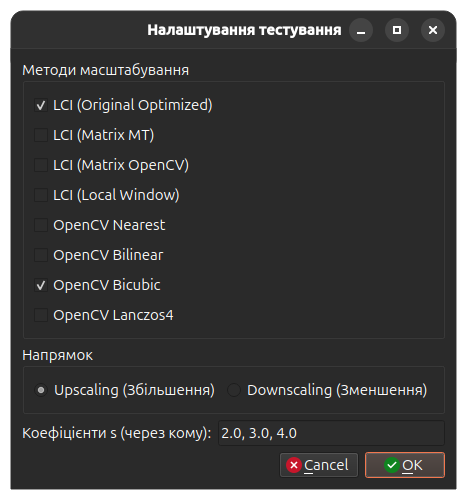
\includegraphics[width=0.6\textwidth]{figures/choseMethods}
	\caption{Вікно налаштування параметрів автоматизованого тестування}
	\label{fig:test_config_dialog}
\end{figure}

\newpage
Інтерфейс вікна конфігурації логічно поділений на три основні блоки:
\begin{enumerate}
	\item \textbf{Вибір алгоритмів:} перелік методів для порівняння. Доступні як чотири реалізації розробленого барицентричного методу (оптимізована, матрична багатопотокова, матрична з використанням OpenCV та локальна), так і три базові індустріальні методи з бібліотеки OpenCV (найближчого сусіда, білінійний та бікубічний).
	\item \textbf{Режим трансформації:} перемикач, що визначає напрямок масштабування (Upscaling або Downscaling).
	\item \textbf{Коефіцієнт $s$:} меню для вибору цілочисельного значення масштабу, яке визначає ступінь геометричної зміни розмірів тестового зображення.
\end{enumerate}

\paragraph{Агрегація результатів.}
Після обробки всіх зображень для поточного методу та коефіцієнта $s$, алгоритм обчислює середнє значення витраченого часу та метрик якості PSNR та SSIM. Отримані середні значення форматуються до заданої кількості знаків після коми та динамічно вставляються як новий рядок у таблицю результатів.